\documentclass[brazil,a4paper,12pt]{article}

\usepackage{fullpage}
\usepackage{fancyvrb}
\usepackage[brazil]{babel}
\usepackage[utf8]{inputenc}
\usepackage{graphicx}
\usepackage{booktabs}

\begin{document}

\begin{center}
\LARGE
\textbf{Mineração de Dados}\\
\textbf{TP1: Tribunal de Contas da União}\\
\end{center}
\begin{center}
\textbf{Aluno: Flavio Vinicius Diniz de Figueiredo}
\end{center}

\section{Descrição}

O objetivo do TP foi de realizar as seguintes três etapas em uma base de dados do Tribunal de Contas da União (TCU):

\begin{description}

\item [Limpeza de dados] Os dados da base original continhas atributos redundantes, difíceis de tratar ou desnecessários. Foi requisitado fazer um limpeza de dados através de técnicas como binificação, discretização, remoção de ruídos etc. Era importante manter em mente que técnicas de padrões frequentes poderiam ser utilizadas para processar os dados (não no TP, mas sim como um cenário fictício).

\item [Geração de novos dados] Após a limpeza de dados, foi requisitado a geração de uma nova base de dados. Os atributos desta nova base poderiam ser um subconjunto dos originais, como também novos atributos derivados dos originais.

\item [Análise da correlação entre características] Utilizando a nova base, foi requisitada uma analise de correlação entre os atributos. 

\item [Definição de métrica para fraudes] Por fim, requisitou-se que fosse proposta uma única métrica capaz de ordenar os vendedores de acordo com um nível de ``fradulencia''. Não foi requisitada a execução desta métrica na base, apenas a proposta da mesma.

\end{description}

\noindent Nas próximas seções vou descrever as quatro etapas.

\section{Limpeza de Dados}

O conjunto de dados originais era composto de 15 atributos, demonstrados na Tabela~\ref{tab:orig}. Apenas os atributos de números $7, 8, 10, 11$ e $12$ são numéricos; os outros são categóricos. A tabela original consiste de $37165$ linhas.

O primeiro passo para limpeza de dados foi considerar apenas os pregões com a situação final (atributo \textsc{Situacao}) como sendo aceito. No total, $6633$ pregões não foram aceitos, os motivos para este fato estão demonstrados na Tabela~\ref{tab:canc}. Pela tabela podemos ver que a maioria dos pregões ou foram cancelados na aceitação, indicando que o valor proposto não era aceitável; ou foram cancelados por inexistência de proposta, indicando que ninguém venceu aquele pregão. Decidi filtrar todos os pregões cancelados como sendo ruído, dado que estes não representam transações de pregão aceitas.


\begin{table}
\centering
\small
\begin{tabular}{clp{10cm}}
\toprule
\# & Nome & Descrição \\
\midrule
1 & \textsc{ChavePregao} & Identificador numérico único de cada pregão \\
\midrule
2 & \textsc{UASG} & Identificador numérico único de cada órgão governamental \\
\midrule
3 & \textsc{PregoeiroOficial} & Nome completo do pregoeiro (i.e., responsável pelo decorrer do leilão) \\
\midrule
4 & \textsc{Descricao} & Descrição textual sucinta sobre o item de compra \\
\midrule
5 & \textsc{DescricaoComplementar} & Descrição detalhada sobre o item de compra \\
\midrule
6 & \textsc{Quantidade} & Quantidade de itens distintos incluídos na compra \\
\midrule
7 & \textsc{UnidadeFornecimento} & Unidade de medida dos itens listados na compra \\
\midrule
8 & \textsc{ValordeReferencia} & Valor total estimado para a compra (em unidade monetárias) \\
\midrule
9 & \textsc{Situacao} & Situação final do pregão \\
\midrule
10 & \textsc{AceitoPara} & Nome do vencedor do pregão \\
\midrule
11 & \textsc{PeloMenorLance} & Valor de compra alcançado ao fim do pregão (em unidade monetárias) \\
\midrule
12 & \textsc{ValorNegociado} & Valor final de compra alcançado após processo de negociação direta entre vencedor do leilão e o pregoeiro \\
\midrule	
13 & \textsc{GanhoNegociacao} & Ganho em unidade monetárias com o processo de negociação \\
\midrule
14 & \textsc{GanhoPregao} & Diferença percentual entre o valor negociado e o valor de referência da venda\\
\midrule
15 & \textsc{AceitoParaCNPJ} & Número CNPJ do vencedor do pregão \\
\bottomrule
\end{tabular}
\caption{Atributos Originais}
\label{tab:orig}
\end{table}

\begin{table}
\centering
\small
\begin{tabular}{cl}
\toprule
Número Cancelados & Motivo  \\
\midrule
52 & Cancelado \\
\midrule
2742 & Cancelado na aceitação \\
\midrule
139 & Cancelado por decisão do pregoeiro \\
\midrule
3152 & Cancelado por inexistência de proposta \\
\midrule
548 & Item deserto \\
\bottomrule
\end{tabular}
\caption{Pregões Cancelados}
\label{tab:canc}
\end{table}

Após o filtro por cancelamento, buscamos ruídos de dados de acordo de acordo com a seguintes regras:

\begin{description}
\item [CNPJ Válidos] Verifiquei se todo CNPJ (atributo \textsc{AceitoParaCNPJ}) era único para cada o vencendo do pregão (atributo \textsc{AceitoPara}). Ou seja, se o nome de cada vencedor de pregão tinha apenas um CNPJ. Apenas um CNPJ foi suspeito de invalidez por essa analise, este exemplo segue abaixo:

\begin{verbatim}
CNPJ 04.499.486/0001-05 ->
         MSKBYTE COMERCIO E MANUTENCAO DE EQUIPAMENTOS PARA INFO
         GLOSSARIO COMERCIO DE LIVROS LTDA - EPP
\end{verbatim}

Também verifiquei se cada pregão foi ganho por um CNPJ apenas, neste caso não encontrei nenhuma linha inválida.

\item [Ganho Correto] Foi também verificado se o valor do atributo \textsc{GanhoPregao} estava de acordo com os atributos \textsc{ValorNegociado} e \textsc{ValordeReferencia}. O ganho é computado da seguinte forma:

$$ GanhoPregao = \frac{ValordeReferencia - ValorNegociado}{ValordeReferencia} * 100 $$

\noindent No total, 1330 linhas tinha o valor de \textsc{GanhoPregao} errados de acordo com a fórmula acima. Estas foram removidas.

\end{description}

\section{Geração de Novos Dados}

O primeiro passo da geração de novos dados foi a remoção de atributos redundantes. É simples de perceber que os atributos \textsc{AceitoPara} e \textsc{AceitoParaCNPJ} são redundantes, por este motivo decidi manter apenas o \textsc{AceitoParaCNPJ}. Além disso, um dos três atributos \textsc{ValorNegociado}, \textsc{ValordeReferencia} e \textsc{GanhoPregao} pode ser removido, dado que com dois destes podemos computar o terceiro. Decidi por remover o \textsc{ValorNegociado}.

Decidi por agrupar 4 atributos \textsc{Descricao}, \textsc{DescricaoComplementar}, \textsc{Quantidade} e  \textsc{UnidadeFornecimento} em um novo atributo. Os quatro atributos contém informação importante sobre os tipos de produtos do pregão; porém por serem compostos de texto livre, os mesmos são de difícil análise na sua forma original. Para a geração do novo atributo fiz uso da clusterização das linhas (pregões) de acordo com os 4 originais. Os seguintes passos foram feitos (para mais detalhes sobre estes passos sugiro a leitura do Capítulo 8 do livro Modern Information Retrieval~\cite{baeza2010modern}):

\begin{enumerate}

\item Agrupar os 4 atributos como sendo uma única string (denominada aqui de documento). Esta técnica é conhecida como \emph{bag-of-words}.

\item Transformar os documentos gerados a acima em vetores. Para isto, os termos foram ponderados por $TF-IDF$~\cite{baeza2010modern}. Após isto é trivial transformar documentos em vetores, sendo cada termo um atributo do documento em forma vetorial.

\item Os documentos foram agrupados usando o algoritmo \emph{K-means}. A métrica de distância entre vetores utilizada foi a euclideana. Observo que algoritmos e métricas de distância mais avançadas poderiam ser utilizadas, porém pela característica exploratória do TP optei pelo mais simples. 

Um dos problemas do uso do \emph{K-means} é a escolha do número de grupos. Para resolver este, executei 20 vezes o algoritmo para diferentes valores número de grupos (k). Após a execução, analisei a razão média entre: (1) a distância entre os centros do grupos; ; com (2) a distância de cada documento para seu grupos. Esta análise está representada na Figura~\ref{fig:clust}, a mesma está descrita com mais detalhes no livro Perfomance by Design~\cite{menasce2004performance}. Pela figura, podemos ver que após $7$ grupos a razão computada estabiliza. Como a ideia do agrupamento é maximizar a distância inter grupos (1) e minimizar as distâncias internas dos grupos (2), pode se dizer que qualquer valor após $7$ tem a mesma qualidade. Por isto, escolhemos como $7$ o número de grupos.

\begin{figure}
\centering
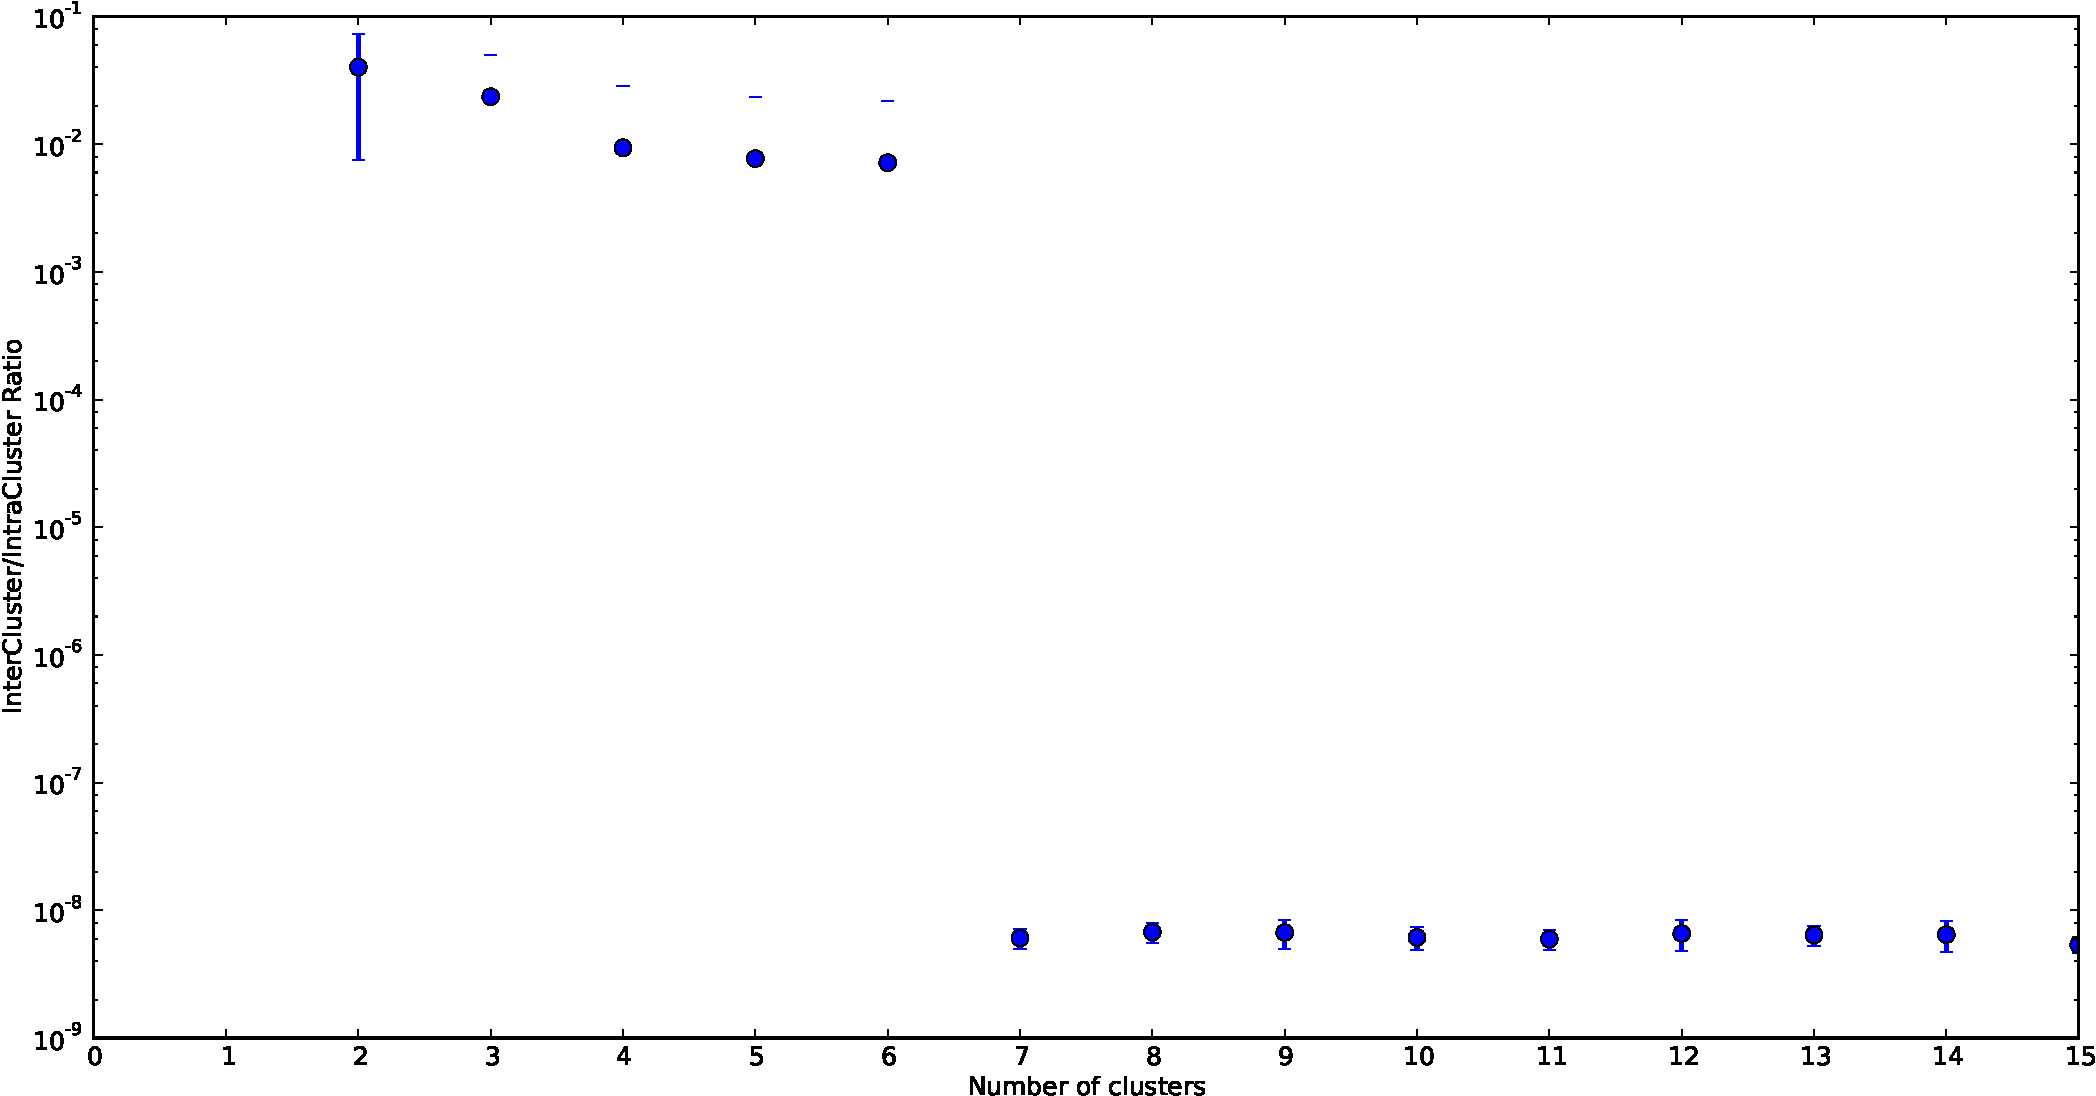
\includegraphics[scale=0.4]{clust-crop.pdf}
\caption{Razão das distâncias intra e inter grupos}
\label{fig:clust}
\end{figure}

\end{enumerate}

Após estes passos, os 4 atributos foram agrupados em um só novo \textsc{Cluster}, que contém o grupo de cada linha. A ideia final do agrupamento é que produtos similares fazem parte do mesmo grupo. O menor grupo foi composto de 170 linhas, enquanto o maior obteve 12220 linhas.

Por fim, criamos um outro novo atributo denominado de \textsc{SuperFaturamento}. Este é a discretização do atributo \textsc{GanhoPregao} (que foi mantido). A ideia aqui é capturar valores discrepantes negociados como um atributo categórico, mais útil para algoritmos de padrões frequentes. O agrupamento foi dado da seguinte forma:

\begin{enumerate}

\item Se o ganho for até $50\%$ a mais do \textsc{ValordeReferencia}, dizemos que não houve super faturamento.

\item Se for entre $500\%$ e $50\%$, indico que o valor é superfaturado.

\item Se for mais que $500\%$, indico que o valor é \textbf{muito} superfaturado.

\end{enumerate}

A Figura~\ref{fig:super} mostra a distribuição de ganhos, por clareza, esta figura não mostra valores abaixo de $500\%$, nosso limiar mais baixo. Após os filtros e conversões, restaram $29202$ linhas para serem analisadas. Destas, $1243$ eram superfaturadas e $290$ eram muito superfaturadas. 

\begin{figure}
\centering
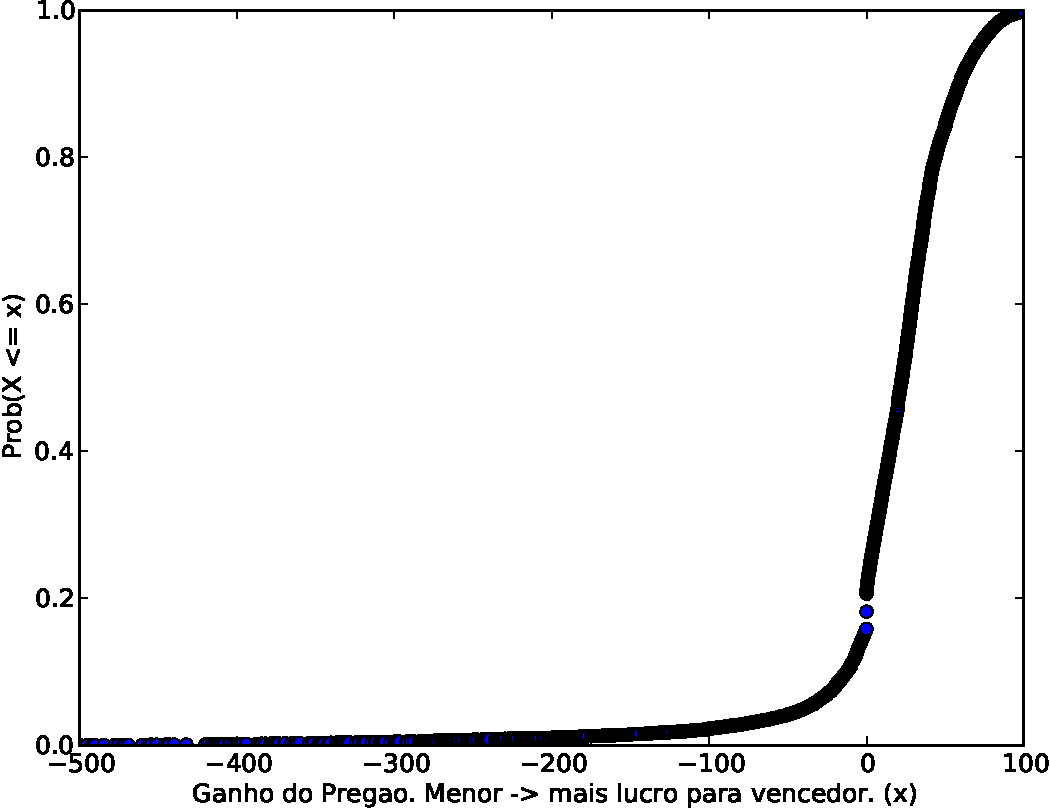
\includegraphics[scale=0.7]{ganho-crop.pdf}
\caption{Distribuição de Ganhos}
\label{fig:super}
\end{figure}

\section{Análise de Correlação}

A terceira etapa do TP consistia em analisar a correlação entre os atributos da nova base, tais correlações foram mensuradas entre pares de atributos. Para compara os atributos numéricos (\textsc{ValordeReferencia}, \textsc{GanhoPregao} e \textsc{PeloMenorLance} fiz uso da correlação de Pearson. Para os atributos categóricos restantes, fiz use do teste $Chi-squared$ descrito no Capítulo 3 do livro da disciplina~\cite{meira}. 

Surpreendentemente, não foi encontrada uma correlação significativa entre os atributos \textsc{ValordeReferencia} e \textsc{GanhoPregao}. Acredito que o motivo para isto é que o \textsc{ValordeReferencia} é um fator que aparecente tanto no denominador como no numerador da equação do \textsc{GanhoPregao}, pois o ganho é percentual. Se mensurarmos entre o atributo \textsc{ValorNegociado} (na base original), a correlação é muito alta (acima de $0.9$); pois como esperado, quando maior o valor negociado maior o lucro. O atributo \textsc{PeloMenorLance} é fracamente correlacionado (correlação de $0.2$) com o \textsc{ValordeReferencia}, que novamente é esperando pois é intuitivo ver que produtos mais baratos tem lances menores.

Não foi encontrada nenhuma correlação estatisticamente válida entre atributos categóricos. Todas, tiverem a hipótese nula de independência sendo aceita ($p-values$ abaixo de 0.01). Acredito que o motivo para este resultado foi a quantidade de zeros nas matrizes de contingência. Não é comum a co-ocorrência de atributos, dado a distribuição viésada de alguns, como \textsc{SuperFaturamento} e \textsc{Cluster}, e a alta quantidade de valores de outros como \textsc{AceitoParaCNPJ}.

\section{Métrica de Fraude}

Uma métrica simples de de fraudulência é a a co-ocorrência de pregoeiros com comprados em pregões super faturados. Por exemplo, analisando os dados, 29 ocorrência de um superfaturamento muito alto (acima $500\%$) foi entre a pregoeira Alexandra ``Ma. Rosas P. da Silva'' com o comprador ``22.805.436/0001-90''. Um outro pregoeiro, ``ALBERTO CARLOS MALHEIROS CARVALHO'', obteve mais de 40 pregões muito superfaturados para 4 CNPJs. A análise desta métrica é trivial após construída a matriz de contingência utilizada para as correlações.

Esta métrica pode ser utilizada para capturar pregoeiros e comprados envolvidos em pregões super faturados. Tanto de forma independente, quanto conjunta, indicando a formação de carteis.

\bibliographystyle{plain}
\bibliography{bibs}


\end{document}
